\section{Graphical Model}

\subsection{Introduction}

\begin{definition}{\textbf{(Types of Graph)}}
    There are several kind of graphs that we can use to model the probability distribution: factor graph, undirected graph, and directed graph. Node corresponds to the random variables and the edge in graph indicates statisical dependence between varible.
\end{definition}

\begin{definition}{\textbf{(Dependencies)}}
    For the random variable $X,Y,V$, where we have:
    \begin{itemize}
        \item \emph{Conditional Independence}: $X\ind Y | V$ iff $P(X | Y, V) = P(X|V)$ provided that $P(Y, V)>0$. We can see that furthermore that:
        \begin{equation*}
            P(X, Y | V) = P(X | Y, V) P(Y| V) = P(X|V)P(Y|V)
        \end{equation*}
        Please note that, this can generalize the symbol to the sets of random variables as:
        \begin{equation*}
            \mathcal{X}\ind\mathcal{Y} | \mathcal{V} = \brackc{X\ind Y | \mathcal{V} : \forall X \in \mathcal{X}, \forall Y \in \mathcal{Y}}
        \end{equation*}
        \item \emph{Marginal Independence}: $X\ind Y$ is equivalent to $X\ind Y | \emptyset$ and $P(X, Y) = P(X)P(Y)$
    \end{itemize} 
\end{definition}

\begin{definition}{\textbf{(Factor Graph)}}
    Factor Graph is a directed graphical representation of the factorized model structure, where each square indicates the factor over the linked variables:
    \begin{equation*}
        P(\mathcal{X}) = \frac{1}{Z}\prod_j f_j(\mathcal{X}_{C_j})
    \end{equation*} 
    where we have the following components:
    \begin{itemize}
        \item $\mathcal{X} = \brackc{X_1,\dots,X_k}$
        \item $\mathcal{X}_S = \brackc{X_i : i \in S}$
        \item $j$ is index that indicates the factor $C_j$ that contains all indicies of variable adjecent to factor $j$
        \item $f_j$ is factor function
        \item $Z$ is normalization constant
    \end{itemize}
    The conditional independent is defined by $X\ind Y | \mathcal{V}$ if every path between $X$ and $Y$ contains some $V\in\mathcal{V}$ (this can be shown that).
\end{definition}

\begin{remark}{\textbf{(Conditional Distribution)}}
    Now, if every path between $X$ and $Y$ contains some $V \in \mathcal{V}$, then there exists a factorization. We have the following joint distribution
    \begin{equation*}
        P(X, Y, \mathcal{V},\dots) = \frac{1}{Z}g_X(X,\mathcal{V}_X,\mathcal{Q}_X) g_Y(Y, \mathcal{V}_Y, \mathcal{Q}_Y)g_R(\mathcal{Q}_R,\mathcal{V}_R)
    \end{equation*}
    where $\mathcal{V}_X,\mathcal{V}_Y,\mathcal{V}_R\subseteq\mathcal{V}$ and the set containing $\mathcal{Q}_X, \mathcal{Q}_Y, \mathcal{Q}_R$ are disjoint. The conditonal is:
    \begin{equation*}
    \begin{aligned}
        P(X|Y, \mathcal{V},\dots) &= \frac{P(X, Y, \mathcal{V},\dots)}{P(Y, \mathcal{V},\dots)} = \frac{\frac{1}{Z}g_X(X,\mathcal{V}_X,\mathcal{Q}_X) g_Y(Y, \mathcal{V}_Y, \mathcal{Q}_Y)g_R(\mathcal{Q}_R,\mathcal{V}_R)}{\sum_{X'}\frac{1}{Z}g_X(X,\mathcal{V}_X,\mathcal{Q}_X) g_Y(Y, \mathcal{V}_Y, \mathcal{Q}_Y)g_R(\mathcal{Q}_R,\mathcal{V}_R)} \\
        &= \frac{g_X(X,\mathcal{V}_X,\mathcal{Q}_X)}{\sum_{X'}g_X(X',\mathcal{V}_X,\mathcal{Q}_X)}
    \end{aligned}
    \end{equation*}
    One the RHS doesn't depend on $Y$ as it follows that $X\ind Y | \mathcal{V}$. 
\end{remark}

\begin{definition}{\textbf{(Markov Blanket)}}
    $\mathcal{V}$ is markov blanket for $X$ iff $X\ind Y | \mathcal{V}$ for all $Y\not\in\brackc{X\cup\mathcal{V}}$
\end{definition}

\begin{remark}
    Each variable $X$ is conditionally independent of all non-neighbourhood given its neighbourhood as we have:
    \begin{equation*}
        X \ind Y | \operatorname{ne}(X) \qquad \forall Y \not\in \brackc{X \cup \operatorname{ne}(X)}
    \end{equation*}
    All neighbourhood $\operatorname{ne}(X)$ is markov blanket of $X$. Please note that it is minimal of such set (markov blanket), which is called \emph{markov boundary}. 
\end{remark}

\begin{definition}{\textbf{(Cliques)}}
    Cliques is fully connected subgraph, whiel the maximal clique is a clique that isn't contains in the other cliques. 
\end{definition}

\begin{definition}{\textbf{(Undirected Graphical Model)}}
    The undirected graphical model is a direct representation of conditional independent and nodes are connected iff they are conditonally dependent given all others. The joint probability factors over maximal clique $C_j$ of the graph is given by:
    \begin{equation*}
        P(\mathcal{X}) = \frac{1}{Z}\prod_jf_j(\mathcal{X}_{C_j})
    \end{equation*}
    We have the following dependencies properties:
    \begin{itemize}
        \item $X \ind Y | \mathcal{V}$ if every path between $X$ and $Y$ contains some node $V \in\mathcal{V}$
        \item Each variable $X$ is conditionally independent of all non-neighbour node given its neighbourhood nodes:
        \begin{equation*}
            X\ind Y | \text{ne}(X) \qquad Y \in \brackc{X \cup \operatorname{ne}(X)}
        \end{equation*}
        And so, the neighbours is a markov blanket. 
    \end{itemize}
\end{definition}

\begin{remark}{\textbf{(Factor Graph vs Undirected Model)}}
    Consider $3$ difference types of graph, we can see that each nodes has same neighbour: 
    \begin{figure}[H]
        \centering
        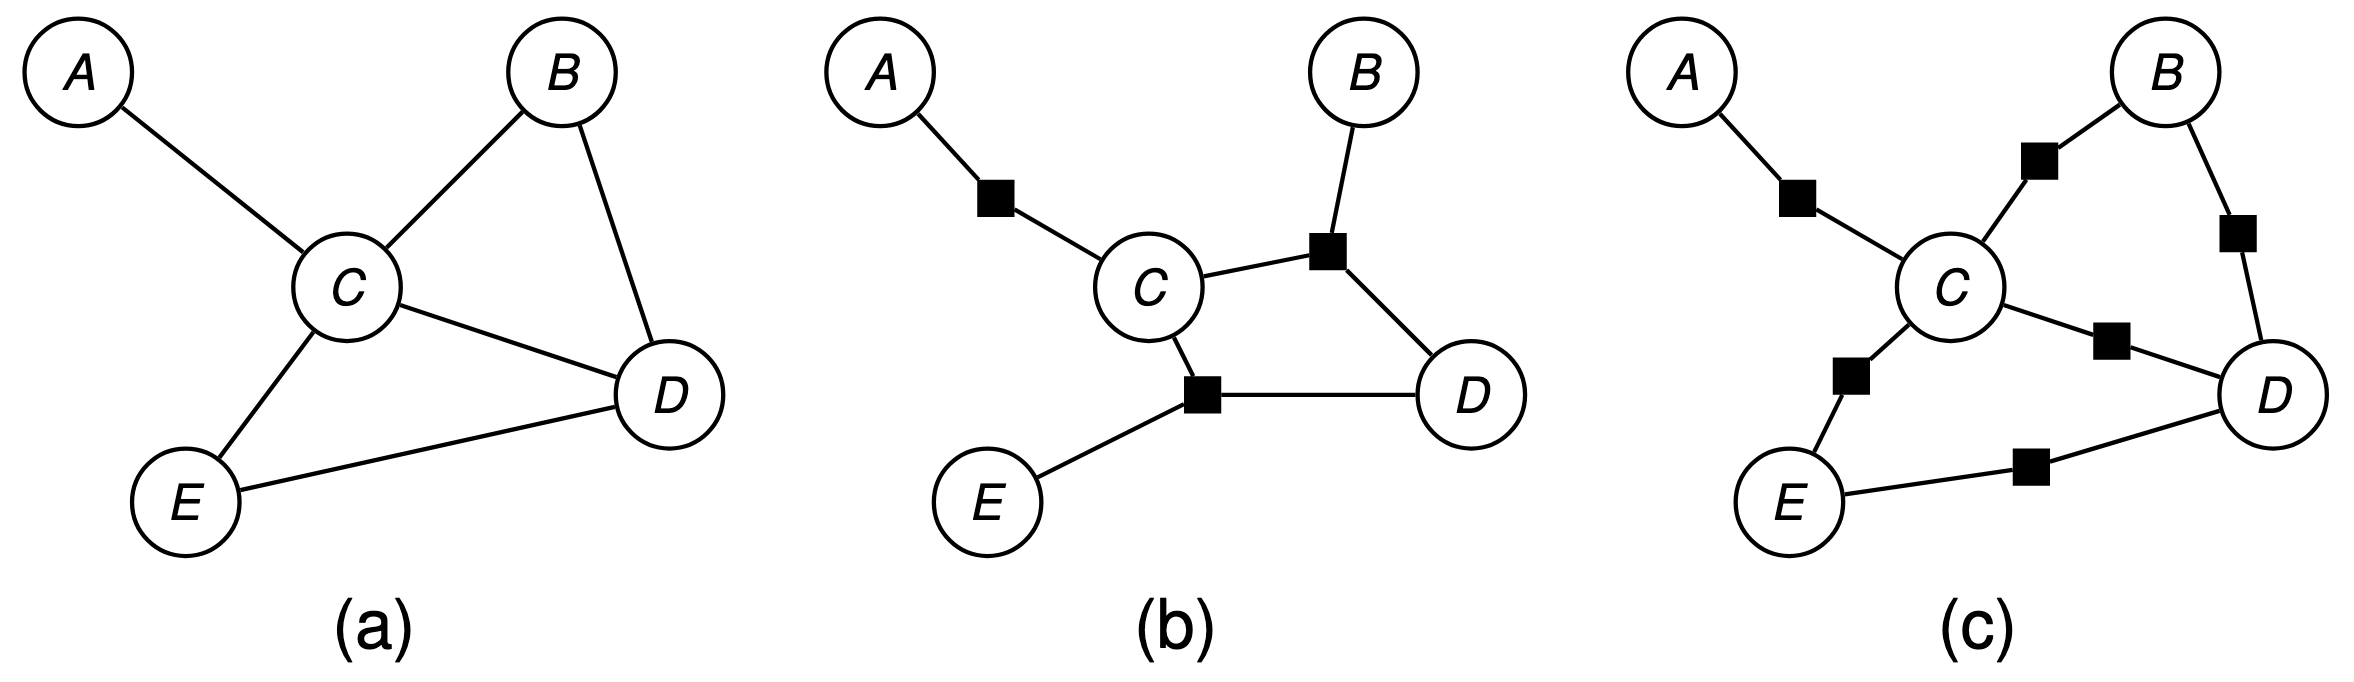
\includegraphics[width=8cm]{img/img1.png}
    \end{figure}  
    Each graph represents exactly the same conditional independent relationship. However, the maximal factorization differs, suppose we have for each variable $K$ possible values:
    \begin{itemize}
        \item $(a)$ can't distiguish between these (we will adopt the $(b)$ to be safe)
        \item $(b)$ has $2$ three-way factor. This is represented in $\mathcal{O}(K^3)$-size table. 
        \item $(c)$ has only pairwise factors. This is represented in $\mathcal{O}(K^2)$-size table. 
    \end{itemize}
    This means that the factor graphs have richer expressive power than undirected graphical models. But the factors can't be determined by testing for conditional independent.
\end{remark}

\begin{remark}{\textbf{(Limitation of Undirected Graphical Model)}}
    Undirected and Factor graph fails to capture the dependencies as the pair of variables that may be connected because they are some other variable that depends on them, for example:
    \begin{figure}[H]
        \centering
        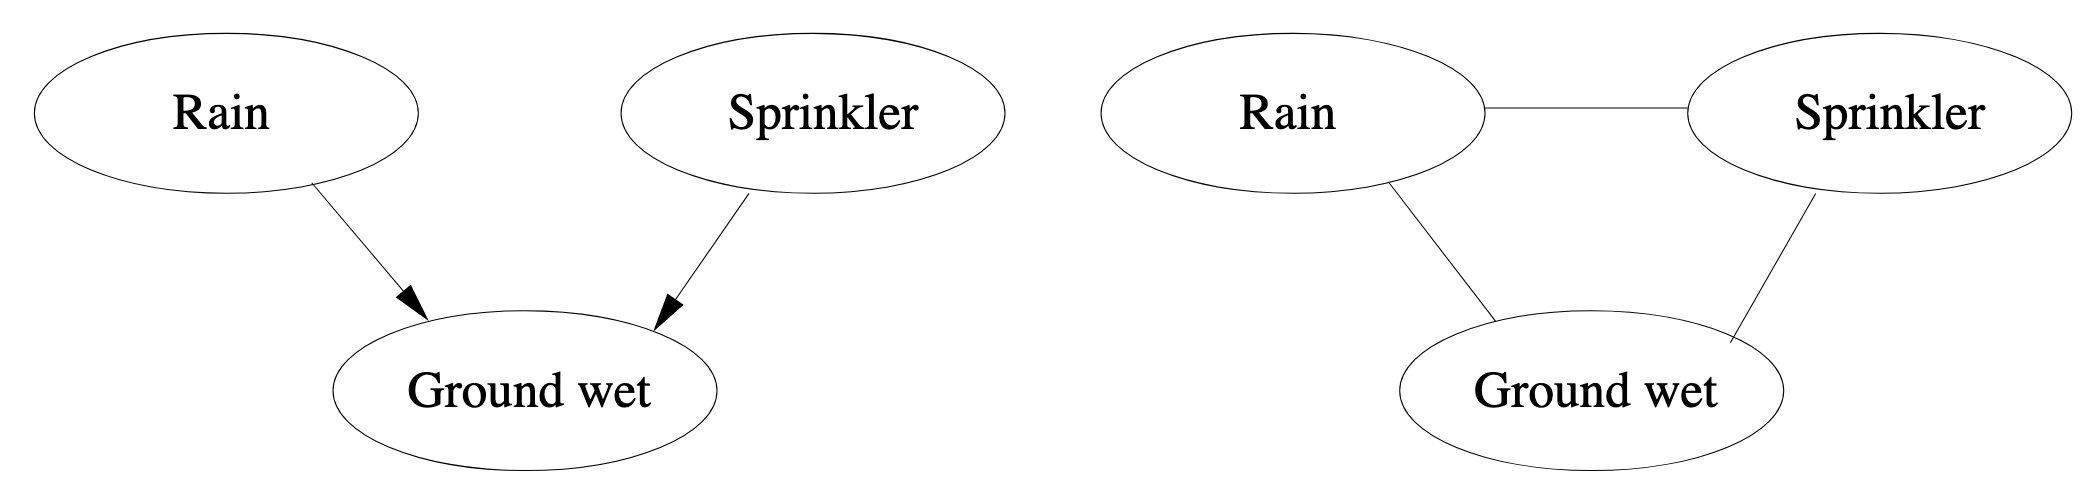
\includegraphics[width=8cm]{img/img2.png}
    \end{figure}  
    If the ground is damped, it may suggest that it was rain, but if we see a sprinkler, then this explain away the damp, thus reduce the our belief of the rain into the prior. For example:
    \begin{equation*}
        R \ind S | \emptyset \quad \text{ but } \quad R\ind S | G
    \end{equation*}
    This is where there is difference between marginal and conditional independent. 
\end{remark}

\begin{definition}{\textbf{(DAG Graphical Model)}}
    A directed acyclic graphical model (DAG) represents a factorization of the joint probability distribution in terms of condtional:
    \begin{equation*}
        P(X_1,\dots,X_n) = \prod^n_{i=1}P(X_i | X_{\text{pa}(i)})
    \end{equation*} 
    where $\text{pa}(\cdot)$ is the parent of node $i$. DAG models are called Baysian network.
\end{definition}

\begin{proposition}
    The conditional Independence between the graph is more complicated than the undirected graph i.e $X\ind Y | \mathcal{V}$. If we consider every undirected path between $X$ and $Y$, the path is blocked by $\mathcal{V}$ if there is a node $V$ on the path such that:
    \begin{itemize}
        \item $V$ has convergnece arrows $\rightarrow V \leftarrow$ on the path and neighbour $V$ nor its descendent are in $\mathcal{V}$
        \item $V$ doesn't have convergnece arrow $\leftarrow V\rightarrow$ or $\rightarrow V \rightarrow$ and $V \in \mathcal{V}$ 
    \end{itemize}
    If all paths are blocked, then $\mathcal{V}$ is $D$-separated between $X$ and $Y$, and so $X\ind Y | \mathcal{V}$. Furthermore, the markov boundary to be:
    \begin{equation*}
        \brackc{\operatorname{pa}(X)\cup\operatorname{ch}(X)\cup\operatorname{pa}(\operatorname{ch}(X))}
    \end{equation*}
\end{proposition}
\begin{proof}
    We can see that the conditional independence of the directed graphical model (for example $A\ind B | \mathcal{D}$) can be modeled as the passing of \correctquote{ball}, in which $2$ variables ($A$, $B$) aren't independence if there is a way that a ball can be passed between them. We will mark the nodes in $\mathcal{V}$ as shaded. There are $10$ simple rules:
    \begin{figure}[H]
        \centering
        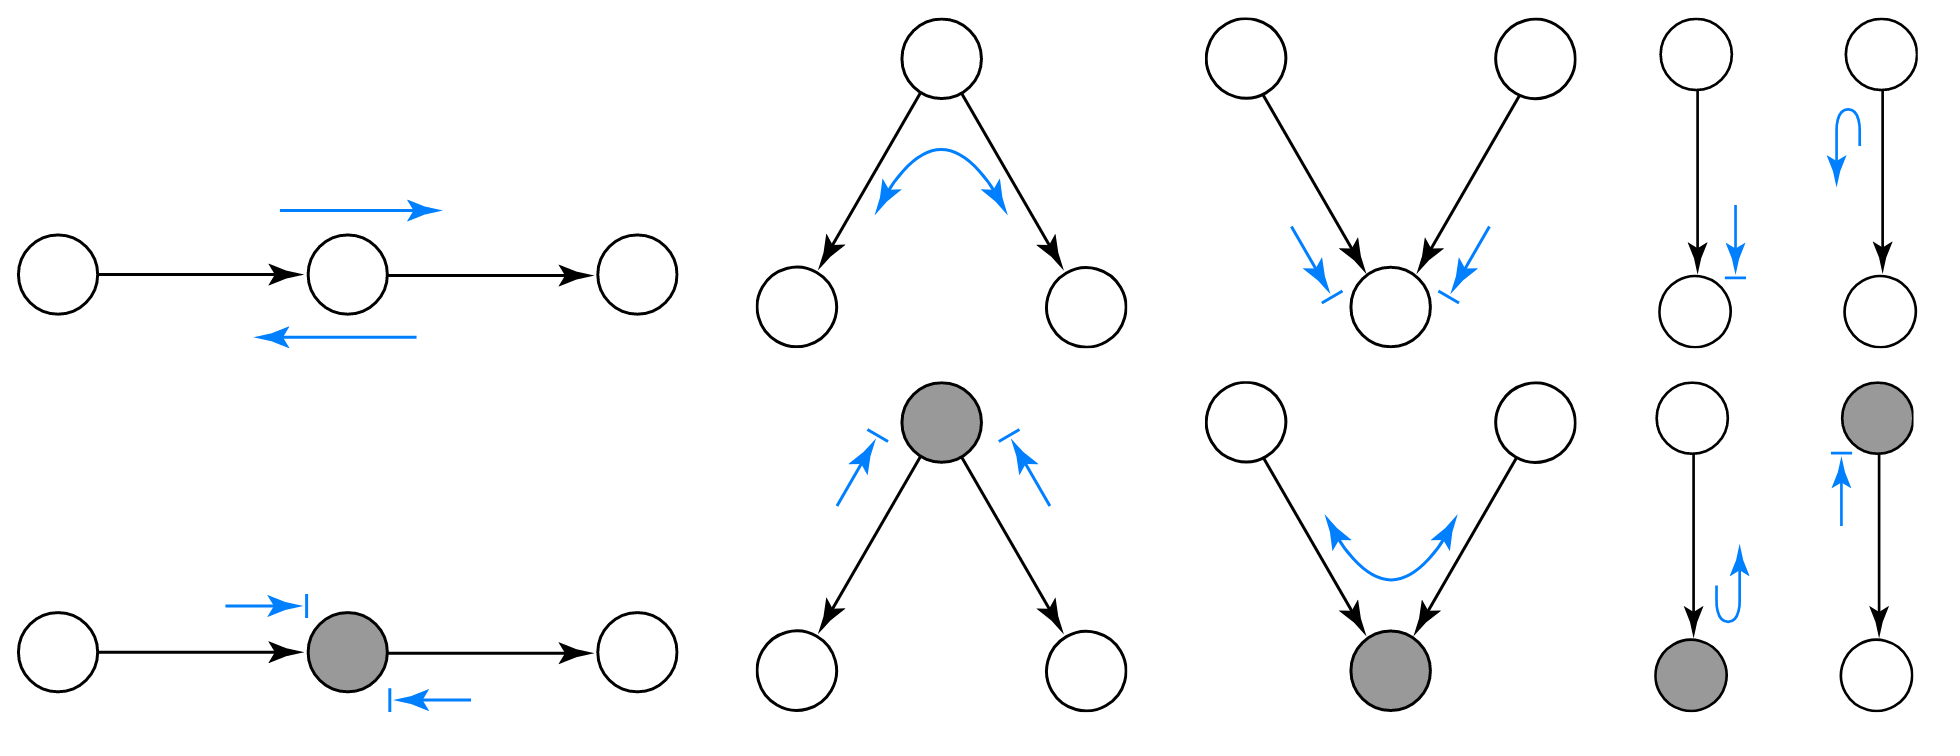
\includegraphics[width=10cm]{img/img3.png}
    \end{figure}  
    Most of the rules are straightforward to see why it is enforced. 
    \begin{itemize}
        \item The first column: Both variables are separated by a middle node, then both of the are independent of each other, thus unable to pass the \correctquote{ball} to each other, meaning that they are independence given the middle node. (This represents the divergence arrow rule)
        \item Similar explaination can be done in the second column of the image. (This also represents the divergence arrow rule)
        \item For the third column (explaining away), we can see that both of the nodes are independence given nothing, however, they becomes dependence once the middle node is shown. This is a reflection of the convergnece arrow rule. 
        \item Finally, the last 2 columns are boundary rule, which is also straightforward to see why it is enforced.
    \end{itemize}
    Thus, we have the reason why the rules above are used. 
\end{proof}

\begin{remark}{\textbf{(Differences Between DAG and Factor Graph)}}
    There are some types of graphs that DAG can represent its probability distribution, which is:
    \begin{figure}[H]
        \centering
        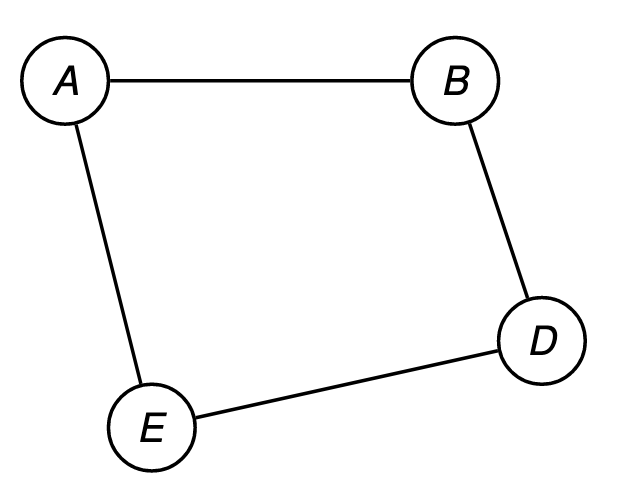
\includegraphics[width=3cm]{img/img4.png}
    \end{figure}  
    This is the only graph that that DAG can't represent. This is because there will always be 2 non-adjecent parent sharing the same child, which implies that:
    \begin{itemize}
        \item The variables are dependence in DAG 
        \item But independence in undirected graph.
    \end{itemize}
    On the other hand, no undirected or factor graph can represent the following DAG and only these:
    \begin{figure}[H]
        \centering
        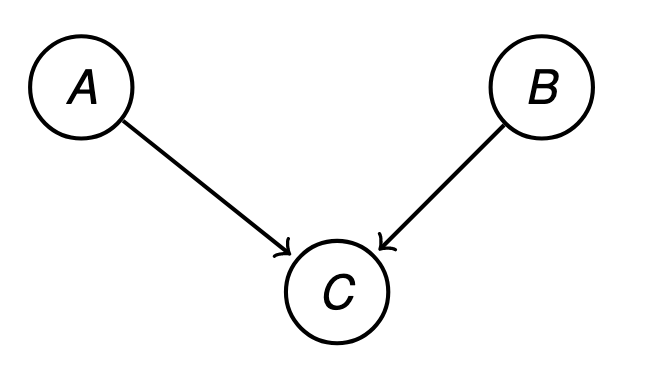
\includegraphics[width=3cm]{img/img5.png}
    \end{figure}  
    This follows from the previous analysis on the explaining away and marginal independence.
\end{remark}

\begin{definition}{\textbf{(Family of Distribution)}}
    Each graph $\mathcal{G}$ implies a set of conditional independence statement: $\mathcal{C}(G) = \brackc{X_i\ind Y_i | \mathcal{Y}}$. Each set $\mathcal{C}$ defines a family of distribution that satisfies all statement in $\mathcal{C}$:
    \begin{equation*}
        P_{\mathcal{C}(G)} = \brackc{P(\mathcal{X}) : P(X_i, Y_i | \mathcal{V}) = P(X_i | \mathcal{V}_i)P(Y_i|\mathcal{Y}_i) \text{ for all } X_i\ind Y_i | \mathcal{V}_i \text{ in } \mathcal{C}  }
    \end{equation*}
    Similarly, we have family distribution in the functional form i.e:
    \begin{equation*}
        P_{G} = \brackc{P(\mathcal{X}) : \frac{1}{Z}\prod_j f_j(\mathcal{X}_{C_j}) \text{ for some non-negative function } f_j }
    \end{equation*}
\end{definition}

\begin{remark}{\textbf{(Family of Distributions)}}
    We can consider the following facts:
    \begin{itemize}
        \item For directed graph: $P_G = P_{\mathcal{C}(G)}$
        \item For undirected graph: $P_G = P_{\mathcal{C}(G)}$ if all distribution are positive i.e $P(\mathcal{X})>0$ for all variable of $\mathcal{X}$
        \item Factor graphs are more expressive as for every undirected graph $G_1$, there is a factor graph $G_2$ such that: $P_{G_1} = P_{G_2}$ but not in other direction.
    \end{itemize}
    Adding edge implies removing conditional independency statement and thus enlarging family of distribution.
\end{remark}

\begin{remark}
    For the next few propositions, we will consider difference kinds of graphical models, which can be shown to interchange with each others:
    \begin{figure}[H]
        \centering
        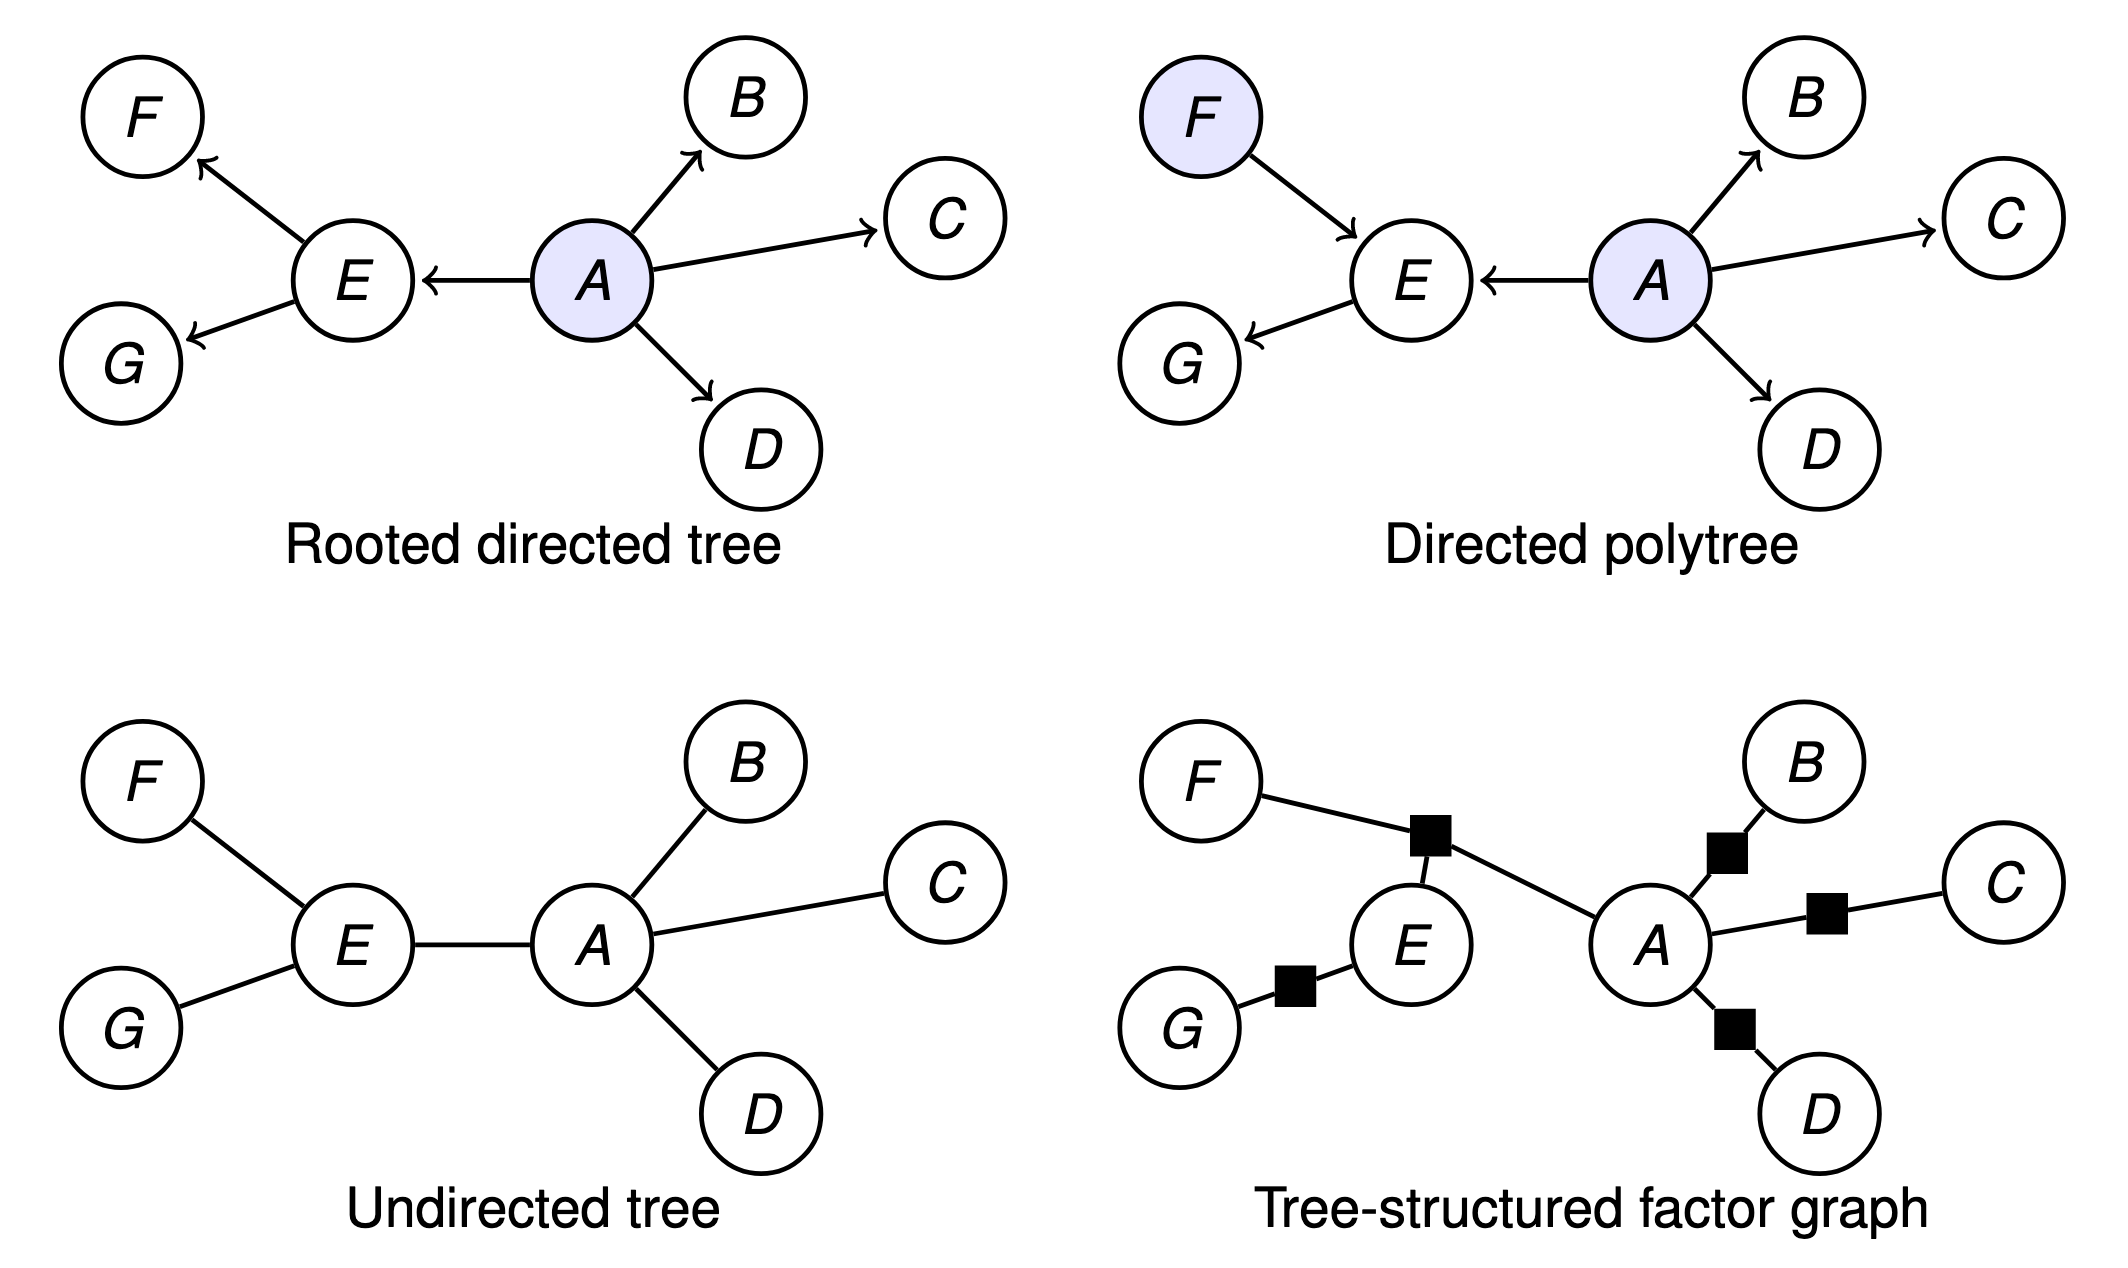
\includegraphics[width=8cm]{img/img6.png}
    \end{figure}  
\end{remark}

\begin{proposition}{\textbf{(Polytree $\boldsymbol \rightarrow$ Tree-Structured Factor Graph)}}
    For DAG that has more than one root, we consider:
    \begin{equation*}
        P(\mathcal{X}) = \prod_i P(X_i | X_{\text{pa}(i)}) =\prod_if_i(X_{C_i})
    \end{equation*} 
    where $C_i = i \cup \operatorname{pa}(i)$ and $f(X_{C_i}) = P(X_i | X_{\operatorname{pa}(i)})$
\end{proposition}

\begin{proposition}{\textbf{(Undirected Tree $\boldsymbol \rightarrow$ Factor Graph)}}
    Since all undirected tree have maximal clique of size $2$, it is equivalent to factor graph with pairwise factor:
    \begin{equation*}
        P(\mathcal{X}) = \frac{1}{Z}\prod_{\operatorname{edge}(i,j)}f_{(i,j)}(X_i, X_j)
    \end{equation*}
\end{proposition}

\begin{proposition}{\textbf{(Rooted Directed Tree $\boldsymbol \rightarrow$ Undirected Tree)}}
    The distribution for single rooted directed tree can be written as a product of pairwise factor of the undirected tree:
    \begin{equation*}
        P(\mathcal{X}) = P(X_r)\prod_{i\ne r}P(X_i | X_{\operatorname{pa}(i)}) = \prod_{\operatorname{edge}(i,j)}f_{(i,j)}(X_i, X_j)
    \end{equation*} 
\end{proposition}

\begin{proposition}{\textbf{(Undirected Tree $\boldsymbol \rightarrow$ Rooted Directed Tree)}}
    Choose arbitary node $X_r$ and set it as a root, which we will point every arrow away from it. Compute the conditional in the DAG as:
    \begin{equation*}
        P(\mathcal{X}) = P(X_r) \prod_{i\ne r}P(X_i|X_{\operatorname{pa}(i)}) = P(X_r)\prod_{i\ne r}\frac{P(X_i, X_{\operatorname{pa}(i)})}{P(X_{\operatorname{pa}(i)})} = \frac{\prod_{\operatorname{edge}(ij)}P(X_i,X_j)}{\prod_{\operatorname{nodes}(i)} P(X_i)^{\operatorname{deg}(i)- 1}}
    \end{equation*}
\end{proposition}

\section{Belief Propagation}

\begin{remark}
    We want to calculate the marginal distribution of a single node $P(X_i)$ and on the edge $P(X_i, X_j)$ based on the undirected graphical model, which we would need to use a belief propagation.
\end{remark}

\begin{proposition}{\textbf{(Marginal Distribution)}}
    The marginal distribution can be calculated locally as:
    \begin{equation*}
        P(X_i) = \prod_{X_j \in \operatorname{ne}(i)} M_{j\rightarrow i} \quad \text{ where } \quad M_{j\rightarrow i} = \sum_{X_j}f_{ij}(X_i, X_j) \prod_{X_k \in \operatorname{ne}(X_j)\backslash\brackc{X_i}} M_{k\rightarrow j}(X_j)
    \end{equation*}
\end{proposition}    
\begin{proof}
    For each neighbourhood $X_j$ of $X_i$ define a disjoint subtree $T_{j\rightarrow i}$ that split by $X_i$:
    \begin{equation*}
    \begin{aligned}
        P(X_i) &= \sum_{\mathcal{X}\backslash\brackc{X_i}} P(\mathcal{X}) \propto \sum_{\mathcal{X}\backslash\brackc{X_i}}\prod_{(i, j)\in \mathcal{E}_T} f_{ij}(X_{i}, X_{j}) \\
        &= \sum_{\mathcal{X}\backslash\brackc{X_i}}\prod_{X_j \in \operatorname{ne}(X_i)}f_{ij}(X_i, X_j)\prod_{(i', j')\in\mathcal{E}_{T_{j\rightarrow i}}}f_{i'j'}(X_{i'}, X_{j'}) \\
        &= \prod_{X_j \in \operatorname{ne}(i)} \bracka{\sum_{\mathcal{X}_{T_{j\rightarrow i}}} f_{ij}(X_i, X_j) \prod_{(i',j')\in\mathcal{E}_{T_{j\rightarrow i}}} f_{i'j'}(X_{i'}, X_{j'}) }
    \end{aligned}
    \end{equation*}
    The last equality comes from the splitting between subtrees, as they are disjoint. $\mathcal{X}_{T_{j\rightarrow i}}$ denotes each edge in the subtree. Let's consider the message:
    \begin{equation*}
    \begin{aligned} 
        M_{j\rightarrow i} 
        &= \sum_{\mathcal{X}_{T_{j\rightarrow i}}} f_{ij}(X_i, X_j) \prod_{(i',j')\in\mathcal{E}_{T_{j\rightarrow i}}} f_{i'j'}(X_{i'}, X_{j'})  \\ 
        &= \sum_{X_j} f_{ij}(X_i, X_j)\sum_{\mathcal{X}_{T_{j\rightarrow i}}\backslash \brackc{X_j}} \prod_{(i',j')\in\mathcal{E}_{T_{j\rightarrow i}}} f_{i'j'}(X_{i'}, X_{j'}) \\
        &= \sum_{X_j} f_{ij}(X_i, X_j) \prod_{X_{k}\in\operatorname{ne}(X_j)\backslash X_i} M_{k\rightarrow i}(X_j)
    \end{aligned}
    \end{equation*}
    The second equality comes from the fact that the factor of $X_i$ is the root of the tree and for any nodes that connection to the factors. If we consider:
    \begin{equation*}
    \begin{aligned}
        \sum_{\mathcal{X}_{T_{j\rightarrow i}}\backslash \brackc{X_j}} \prod_{(i',j')\in\mathcal{E}_{T_{j\rightarrow i}}} f_{i'j'}(X_{i'}, X_{j'}) &\propto P_{T_{j\rightarrow i}}(X_j) \\
        &\propto \prod_{X_{k}\in\operatorname{ne}(X_j)\backslash X_i} M_{k\rightarrow i}(X_j)
    \end{aligned}
    \end{equation*}
    This is due to recursive property of the message passing.
\end{proof}

\begin{proposition}{\textbf{(Pairwise Marginal)}}
    \begin{equation*}
        P(X_i, X_j) = f_{ij}(X_i,X_j)\prod_{X_k \in \operatorname{ne}
        (X_j)\backslash \brackc{X_i} }M_{k\rightarrow j}(X_j) \prod_{X_k\in\operatorname{ne}(X_i)\backslash\brackc{X_j}} M_{k\rightarrow i}(X_i)
    \end{equation*}
\end{proposition}
\begin{proof}
    We consider:
    \begin{equation*}
    \begin{aligned}
        P(X_i, X_j) &= \sum_{X\backslash\brackc{X_i, X_j}}P(\mathcal{X}) \propto \sum_{X\backslash\brackc{X_i, X_j}}\prod_{(i,j)\in\mathcal{E}_T}f_{ij}(X_i, X_j) \\
        &= \sum_{X\backslash\brackc{X_i, X_j}}f_{ij}(X_i, X_j)\prod_{(i'j')\in\mathcal{E}_{T_{j\rightarrow i}}}f_{i'j'}(X_{i'}, X_{j'})\prod_{(i'j')\in\mathcal{E}_{T_{i\rightarrow j}}}f_{i'j'}(X_{i'}, X_{j'}) \\
        &= f_{ij}(X_i, X_j)\bracka{\sum_{\mathcal{X}_{T_{j\rightarrow i}}} \prod_{(i'j')\in\mathcal{E}_{j\rightarrow i}} f_{i'j'}(X_{i'}, Y_{j'}) }\bracka{ \sum_{\mathcal{X}_{T_{i\rightarrow j}}}\prod_{(i'j')\in\mathcal{E}_{T_{i\rightarrow j}}} f_{i'j'}(X_{i'}, Y_{j'}) } \\
        &= f_{ij}(X_i,X_j)\prod_{X_k \in \operatorname{ne}
        (X_j)\backslash \brackc{X_i} }M_{k\rightarrow j}(X_j) \prod_{X_k\in\operatorname{ne}(X_i)\backslash\brackc{X_j}} M_{k\rightarrow i}(X_i)
    \end{aligned}
    \end{equation*}
\end{proof}

\begin{remark}{\textbf{(Belief Propagation for Inference)}}
    Let's consider the belief propagation for inference on the following graphical model:
    \begin{figure}[H]
        \centering
        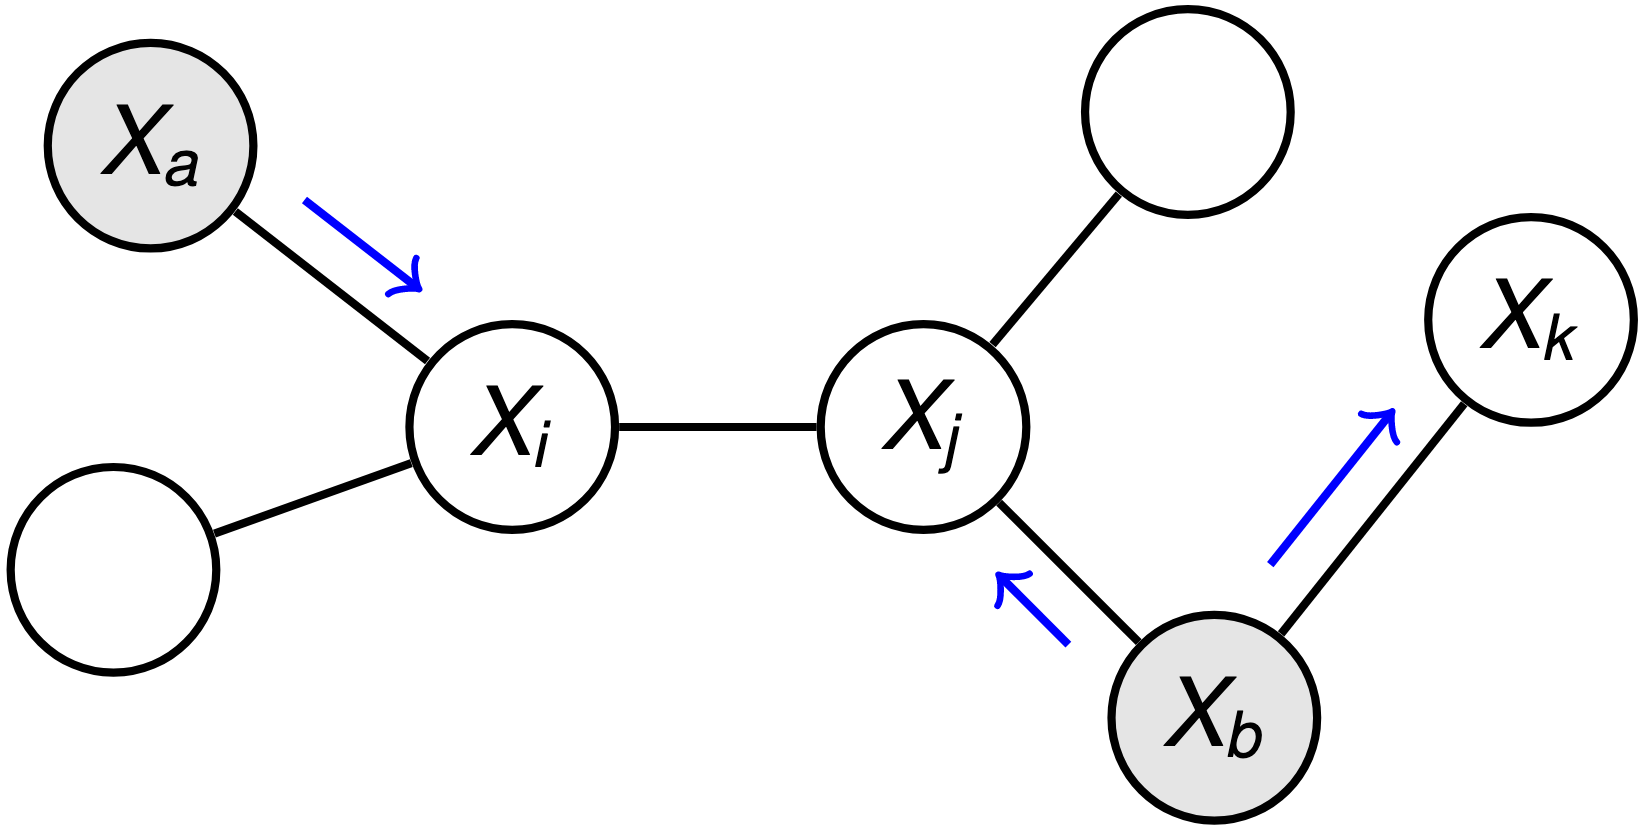
\includegraphics[width=8cm]{img/img7.png}
    \end{figure}  
    To compute the $P(X_i | X_a = a)$ as we have the following message:
    \begin{equation*}
        M_{a\rightarrow i} = f_{ai}(X_a = a, X_i)
    \end{equation*}
    Please note that computing $P(X_i)$ requires that $M_{a\rightarrow i} = \sum_{X_a}f_{ai}(X_a, X_i)$. 
    For the internal node that partition the graph, like variable like $X_b$, we have the following message:
    \begin{equation*}
        M_{b\rightarrow j} = f_{bj}(X_b = b, X_j) \qquad M_{b\rightarrow k} = f_{bk}(X_b = b, X_k)
    \end{equation*}
    Please note that $M_{i\rightarrow j}$ are proportional to likelihood based on any observed variable (within message subtree) and possibly scaled by the prior (depends on factorization):
    \begin{equation*}
        M_{i\rightarrow j}(X_j) \propto P(\mathcal{X}_{T_{i\rightarrow j}}\cap\mathcal{O} | X_j)P(X_j)
    \end{equation*}
    If we consider the message to the observed node, then we have the likelihood. Keeepin all messages unnormalize and any marginal, then the normalizer is the likelihood. 
\end{remark}

\begin{remark}{\textbf{(BP Latent Chain Model)}}
    We consider the belief propagation in the latent chain model, which is a rooted directed tree, as we have the following graphical model:
    \begin{figure}[H]
        \centering
        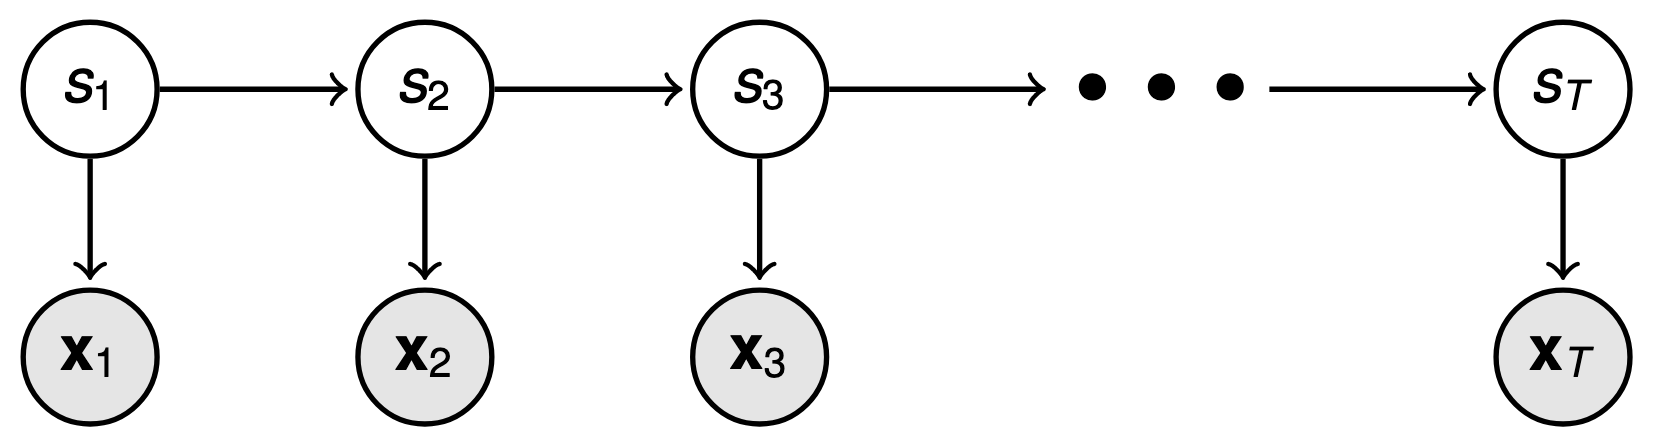
\includegraphics[width=8cm]{img/img8.png}
    \end{figure}  
    We use the backward-forward algorithm is just belief propagation on this graph:
    \begin{itemize}
        \item $\alpha_t(i) = M_{s_{t-1}\rightarrow s_t}(s_t = i) \propto P(x_{1:t}, s_t)$ 
        \item $\beta_t(i) = M_{s_{t+1}\rightarrow s_t}(s_t = i)\propto P(x_{t+1: T} | s_t)$
    \end{itemize}
    where we can easily see that:
    \begin{equation*}
        \alpha_t(i)\beta_t(i) = \prod_{j\in\operatorname{ne}(s_t)} M_{j\rightarrow s_t}(s_t = i) \propto P(s_t = i | \mathcal{O}) 
    \end{equation*}
    The algorithm like BP extend the power of graphical model beyound just encoding of independent and factorization. A single derivation surves multiple models.
\end{remark}

\subsection{Junction Tree}

\begin{remark}{\textbf{(Inference on Graph)}}
    The graphical model sometimes, which is represented by an undirected graph isn't a tree as we would like to find the marginal probability of the single value. There are several strategies that we can use:
    \begin{itemize}
        \item Propagate the local message anyway and hope for the best. This is called \correctquote{loopy belief propagation}, which is an approximation technique. 
        \item Grouping the variable together with multi-variable nodes until the resulting graph, which is a tree as we are going consider this. 
    \end{itemize}
\end{remark}

\begin{remark}{\textbf{(Transforming the Graph)}}
    Consider to transform the graph into one that is easier to handle. As the original graph $G$ encodes a distribution $P(\mathcal{X})$ with a certain factorization or independent structure:
    \begin{itemize}
        \item Transformation from $G$ into an easy to handle $G'$ as it will be valid if $P(\mathcal{X})$ can be represented by $G'$
        \item Ensuring this, we need every step of the graph transformation only to remove condtional independence (never adding them).
        \item Making the family of possible encoding distribution groups grows or stay the same at each step. 
        \item The factor potential on the new graph $G'$ are built from those given on $G$ as to make sure it encodes the same distribution.  
    \end{itemize}    
\end{remark}

\begin{definition}{\textbf{(Junction Tree)}}
    A junction tree is a tree whose node and edges are labelled with set of variables. 
    \begin{itemize}
        \item Each node is represented by a cliques, edges are labelled by intersection of cliques called seperator. 
        \item The cliques contains all adjacent separator. 
        \item Furthermore, if $2$ cliques contain variable $X$, all cliques and separator on the path between $2$ cliques must contain $X$
    \end{itemize}
\end{definition}

\begin{definition}{\textbf{(Constructing Junction Tree)}}
    We consider the following step that transform DAG into a junction tree, which is shown in the figure below:
    \begin{figure}[H]
        \centering
        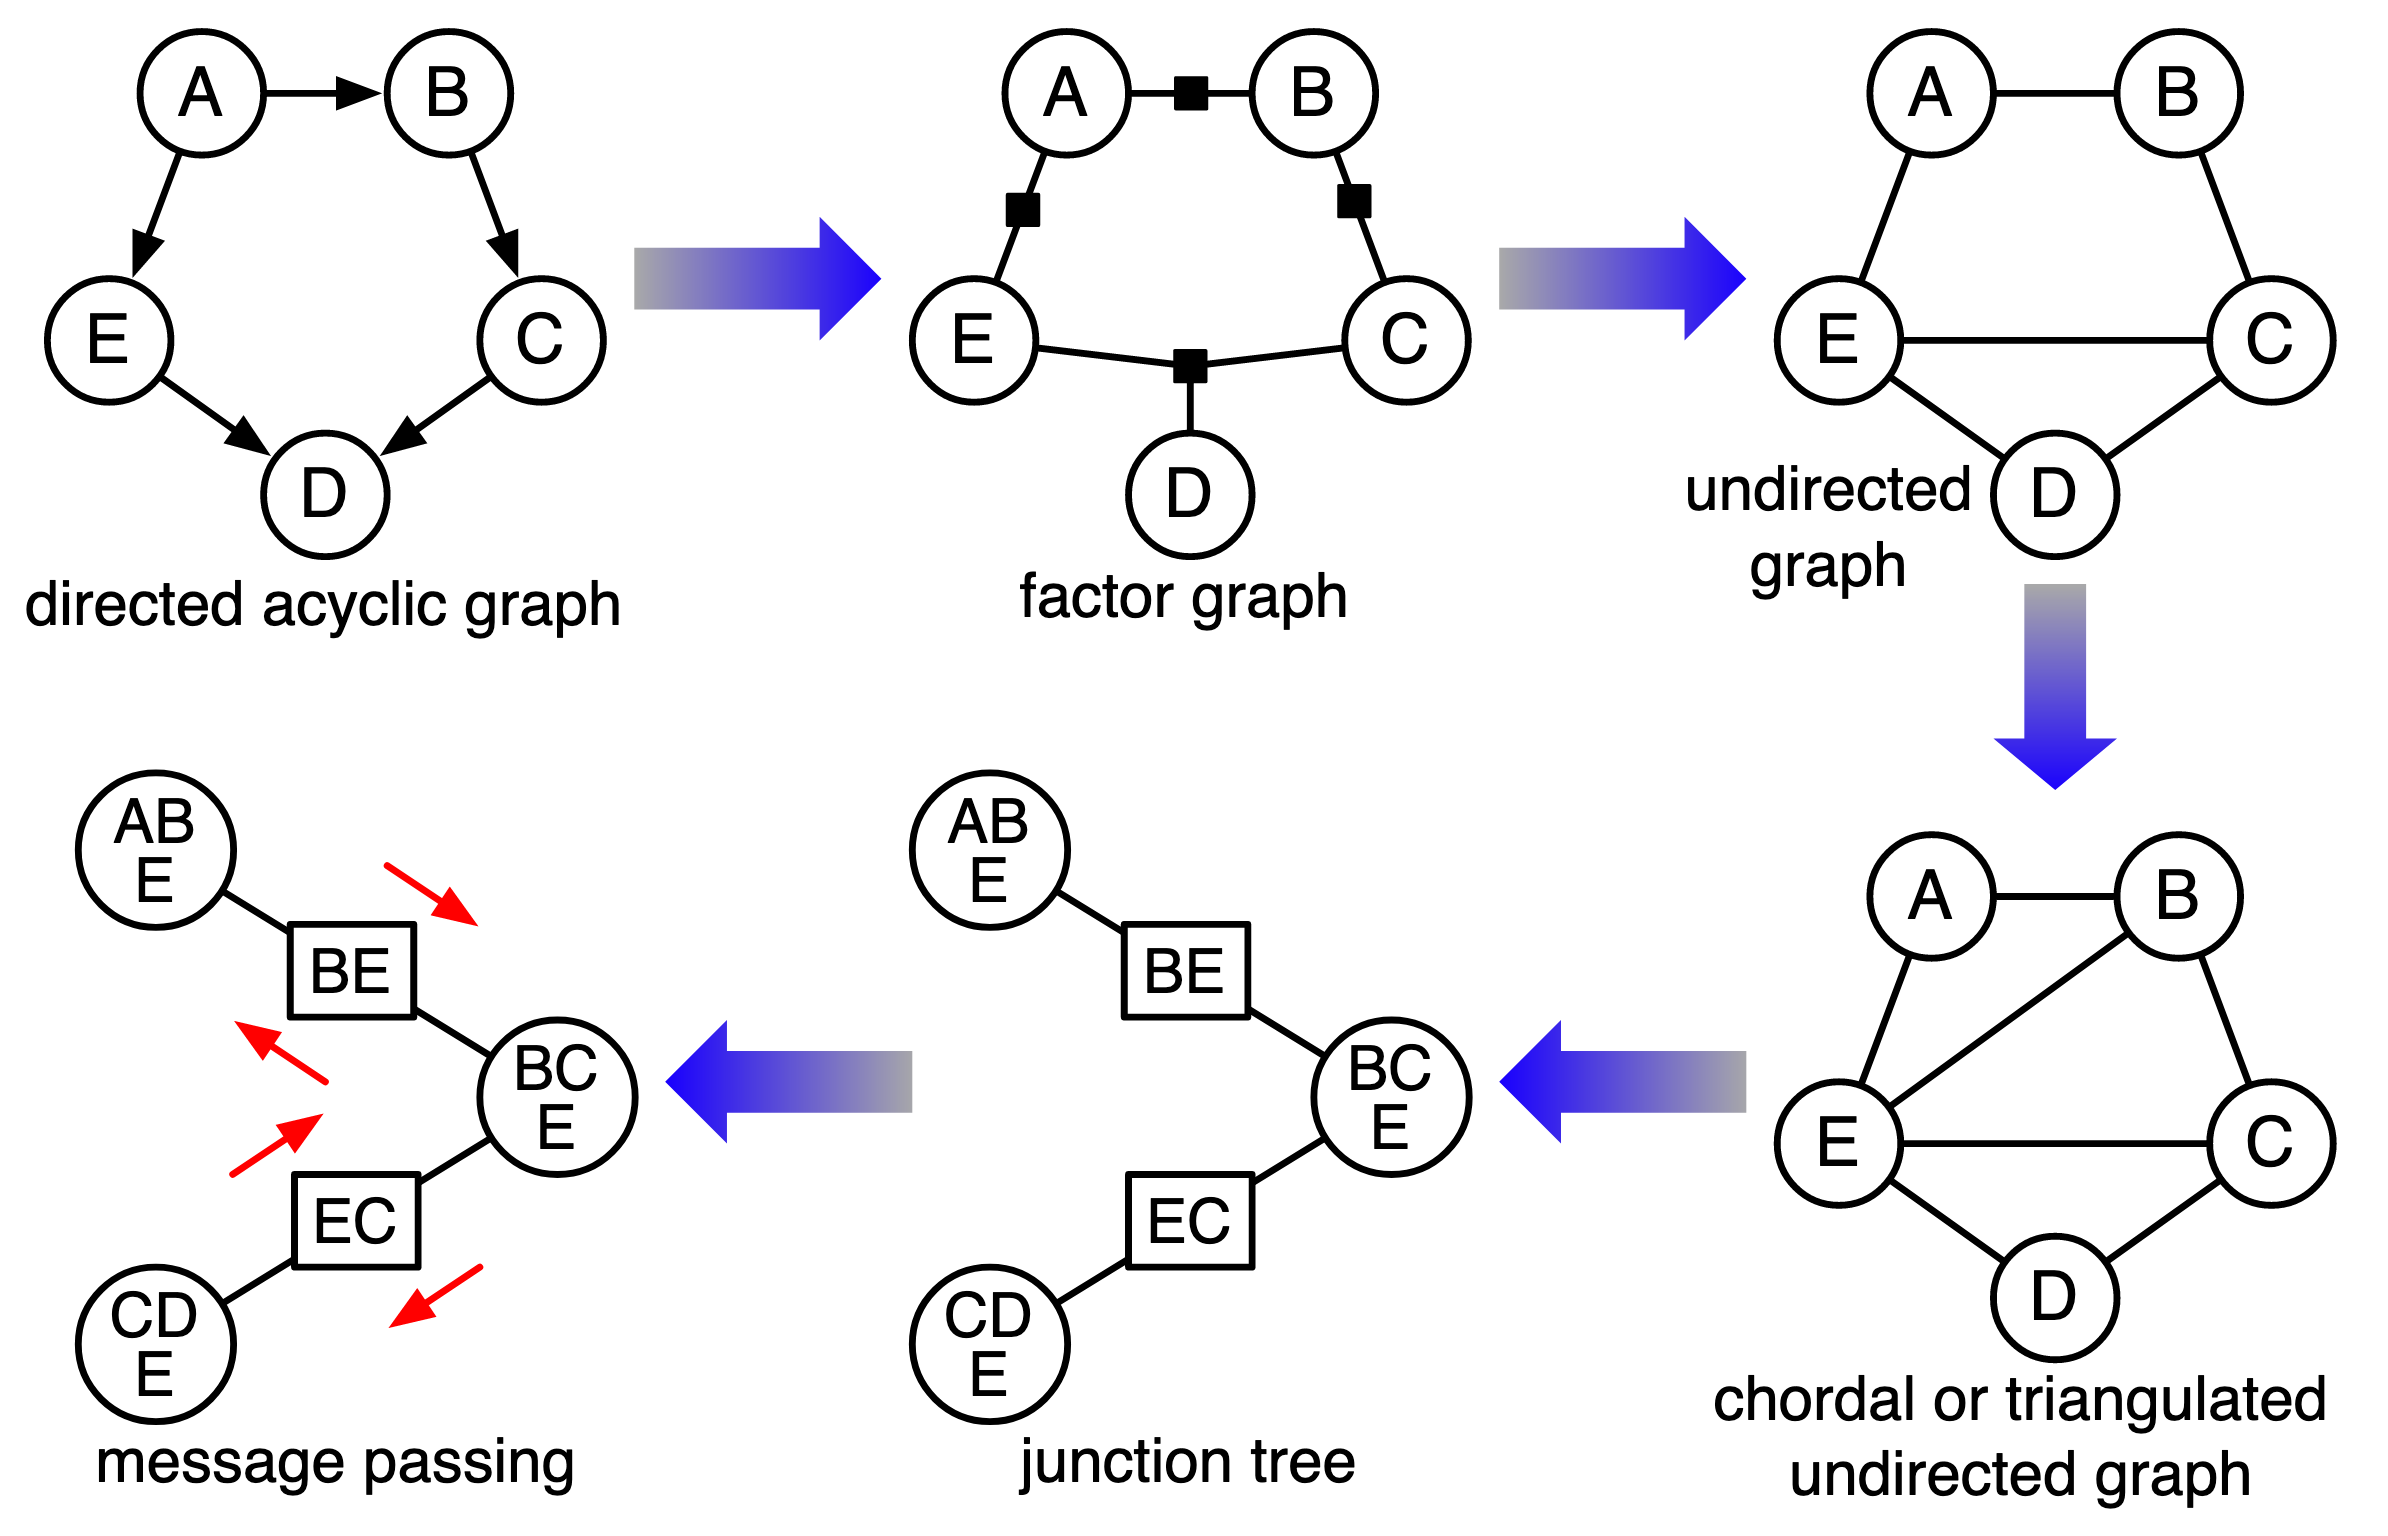
\includegraphics[width=8cm]{img/img9.png}
    \end{figure}  
    There are many process that we have to perform. 

    \textbf{DAG to Factor Graph:} The factor can be see as the conditional distribution of DAG via:
    \begin{equation*}
        P(\mathcal{X}) = \prod_iP(X_i|X_{\operatorname{pa}(i)}) = \prod_if_i(X_C)
    \end{equation*}
    where $C_i = i\cup \operatorname{pa}(i)$ and $f_i(X_{C_i}) = P(X_i|X_{\operatorname{pa}(i)})$. Marginal distribution on roots $P(X_r)$ absorbed into an adjacent factor.

    \textbf{Observation in Factor Graph:} Usually, inference target a posterior marginal given a set of observed values $P(X_l|\mathcal{O})$; for example, $P(A | D =\text{wet}, C = \text{rain})$. Modify the factor linked to the observed node, or add single factor adjacent to the observed node:
    \begin{equation*}
        f_D(D) = \begin{cases}
            1 &\text{ if } D = \text{wet} \\
            0 &\text{ otherwise }
        \end{cases} \qquad f_C(C) = \begin{cases}
            1 &\text{ if } C = \text{rain} \\
            0 &\text{ otherwise }
        \end{cases}
    \end{equation*}
    
    \textbf{Factor Graph to Undirected Graph:} The trasnformation from DAG to undirected graph is called moralization, where: Marry all parents of each node by adding an edge to connect them. We also drop arrows on all edges. 

    \textbf{Triangulate the Undirected Graph:} Want every factor of DAG must be contained within a maximal cliques of the undirected graph. We will have to perform the following modification:
    \begin{itemize}
        \item Replace each factor by an undirected cliques. 
        \item Construct the potential on each maximal clique by multiplying together factor potential that fall on it, and ensure each factor potential only appear once. 
    \end{itemize}
    To do this, we shall modify the graph as:
    \begin{itemize}
        \item We join the loop into cliques, which can be very inefficient. 
        \item Triangulation is performed to add edges to graph, so that every loop of size $\ge4$ has at least one chord. We will adding it recursively to ensure that the loop $\ge4$ has chords too. 
        \item The graph where every loop of size $\ge4$ has at least one chord is called chordal or triangulated. 
        \item Adding the edge removes conditional independencies, which enlarge the family of distribution. 
    \end{itemize}
    To find the triangulation is NP-complete problem, so we resort to heuristic called variable elimination. Let's consider the order of elimination as we have:
    \begin{equation*}
    \begin{aligned}
        P(X_{(n)}) &= \sum_{X_{\sigma(n-1)}}\cdots\sum_{X_{\sigma(1)}} P(\mathcal{X}) \\
        &= \frac{1}{Z}\sum_{X_{\sigma(n-1)}}\cdots\sum_{X_{\sigma(1)}} \prod_i f_i(\mathcal{X}_{C_i}) \\
        &= \frac{1}{Z}\sum_{X_{\sigma(n-1)}}\cdots\sum_{X_{\sigma(2)}}\prod_{j : C_j \ni \sigma(2)}f_j(\mathcal{X}_{C_j})\sum_{X_{\sigma(1)}} \prod_{i:C_i\ni\sigma(1)}f_i(\mathcal{X}_{C_i}) \\
        &= \frac{1}{Z}\sum_{X_{\sigma(n-1)}}\cdots\sum_{X_{\sigma(2)}}\prod_{j : C_j \ni \sigma(2)}f_j(\mathcal{X}_{C_j})f_\text{new}(\mathcal{X}_\text{new})
    \end{aligned}
    \end{equation*}
    Please note that $C_\text{new}$ is the neighbour of $X_{\sigma(1)}$ and \emph{edges are added to graph connected all nodes in} $C_\text{new}$:
    \begin{itemize}
        \item The graph including of all edges would be induced by elimination is chordal. 
        \item Finding a good triangulation depends on findinga good order of elimination $\sigma(1),\dots,\sigma(n)$. 
        \item It is NP-complete to find the best heuristic, as there are $2$ ways that we pick the next varaible to elimiate as follows:
        \begin{itemize}
            \item Min-Deficiency Search: Choose variable that induces the fewest new edge. 
            \item Max-Cardinal Search: Choose node with most previous visited neighbour.
        \end{itemize}
        In most experiments, min-deficiency search seem empirically be better. 
    \end{itemize}
    \textbf{Chordal Graph to Junction Tree:} To build a junction tree, we follows the procedure as we have:
    \begin{itemize}
        \item Find the maximal clique $C_1,\dots,C_k$ of the chordal undirected graph. 
        \item Create a weighted graph, which nodes are labelled by maximal cliques and edges connected each pair of cliques that shares variables. 
        \item Create an edge with size of separator as we find maximal weight spanning tree of weighted graph. 
    \end{itemize}
    Thus, we have the junction tree.
\end{definition}

\begin{remark}{\textbf{(Junction Tree Figures)}}
    The joint distribution factors over junction tree is:
    \begin{equation*}
        P(\mathcal{X})  = \frac{1}{Z}\prod_if_i(X_{C_i}) = \dots f_\text{ABC}(A, B, C)f_\text{BCD}(B, C, D)\dots
    \end{equation*}
    This violates the usual undirected tree sematics of factor per edge, and so we add the following constriants:
    \begin{itemize}
        \item Introducing the copy of the same variable so that there is no overlaps. 
        \item Adding new delta function that enforce consistency:
        \begin{equation*}
            P(\mathcal{X}) = \dots f_\text{ABC}(A, B^{(1)}, C^{(1)})\underbrace{\delta(B^{(1)} - B^{(2)})\delta(C^{(1)}, C^{(2)})}_{f_\text{sep}(B^{(1)}, C^{(1)}, B^{(2)}, C^{(2)})}f_\text{BCD}(B^{(2)}, C^{(2)}, D)\dots
        \end{equation*}
    \end{itemize}
    Having a new message passing the junction to be:
    \begin{itemize}
        \item Unshared Variable $X^{(-)}_{C_i} = X_{C_i \backslash \bigcup S_{ik}}$
        \item Variable incoming separator $X^{(2)}_{S_{ki}}$ (Same as matching variable $X^{(1)}_{S_{ki}}$ in $k\in\operatorname{ne}(i)\backslash j$)
        \item Variable outgoing separator $X^{(1)}_{S_{ij}}$ (Same as matching varaible $X^{(2)}_{S_{ij}}$ in clique $j$)
        \item The variable that appear in more than one separator will need additional copies.
    \end{itemize}
    The overall process is shown in the following junction tree figure:
    \begin{figure}[H]
        \centering
        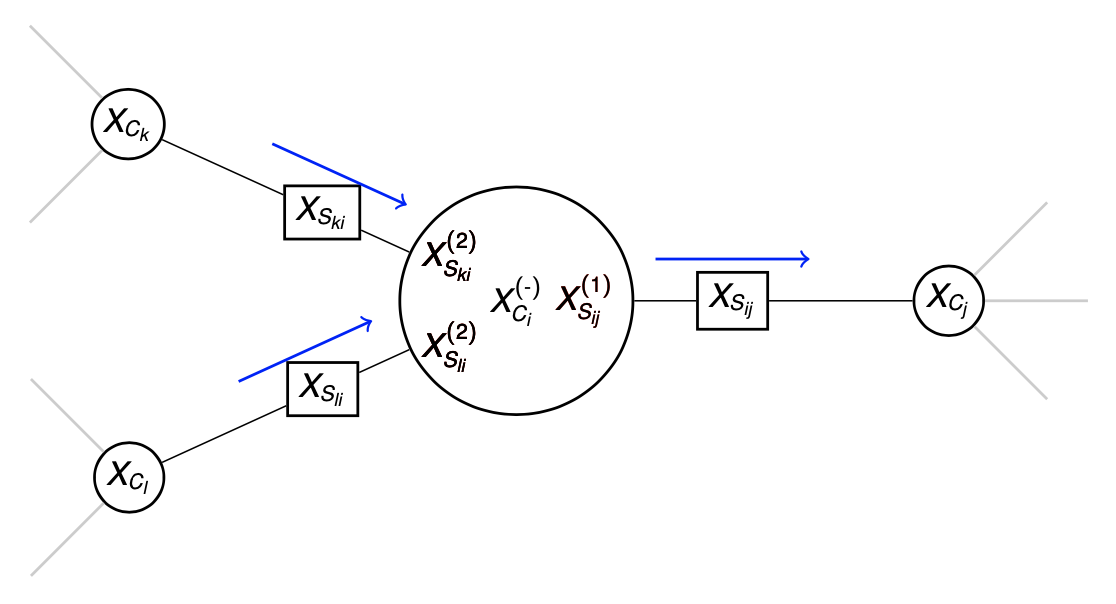
\includegraphics[width=10cm]{img/img10.png}
    \end{figure}  
\end{remark}

\begin{definition}{\textbf{(Shafer-Shenopy)}}
    We have the following formula of the message:
    \begin{equation*}
    \begin{aligned}
        M_{i\rightarrow j}(X^{(2)}_{S_{ij}}) &= \sum_{ X^{(-)}_{C_i}, \brackc{X^{(2)}_{S_{ki}} }, S^{(+)}_{S_{ij}} } f_i\bracka{X^{(-)}_{C_i}, \brackc{X^{(2)}_{S_{ki}} }, S^{(+)}_{S_{ij}} } f_{ij}\bracka{X^{(1)}_{S_{ij}}, X^{(2)}_{S_{ij}}} \prod_{k\in\operatorname{ne}(i)\backslash j} M_{k\rightarrow i}(X^{(2)}_{S_{ij}}) \\
        &= \sum_{X_{C_i}\backslash S_{ij}}f_i(X_{C_i}) \prod_{k\in\operatorname{ne}(i)\backslash j} M_{k\rightarrow i}(X_{S_{ij}}) \\
    \end{aligned}
    \end{equation*}
    The marginal distribution on cliques and separator are defined by:
    \begin{equation*}
    \begin{aligned}
        P(X_{C_i}) \propto f_i(X_{C_i})\prod_{k\in\operatorname{ne}(C_i)}M_{k\rightarrow i}(X_{S_{ki}}) \qquad P(X_{S_{ij}}) \propto M_{i\rightarrow j}(X_{S_{ij}})M_{j\rightarrow i}(X_{S_{ij}})
    \end{aligned}
    \end{equation*}
\end{definition}

\begin{remark}{\textbf{(Junction Tree Properties)}}
    The running intersection property and tree structure of the junction tree implies that local consistency between cliques and separator marginal gurantee global consistency: If we consider the distribution $q_i(X_{C_i})$ and $r_{ij}(X_{S_{ij}})$ are distribution such that:
    \begin{equation*}
        \sum_{X_{C_i\backslash S_{ij}}} q_i(X_{C_i}) = r_{ij}(X_{S_{ij}})
    \end{equation*}
    This implies that that joint distribution to be:
    \begin{equation*}
        P(\mathcal{X}) = \frac{\prod_{\text{cliques } i} q_i(X_{C_i})}{\prod_{\text{separator } (ij)} r_{ij}(X_{S_{ij}})}
    \end{equation*}
    As we have:
    \begin{equation*}
        q_i(X_{C_i}) = \sum_{\mathcal{X}\backslash X_{C_i}}P(\mathcal{X}) \qquad r_{ij}(X_{S_{ij}}) =  \sum_{\mathcal{X}\backslash X_{S_{ij}}}P(\mathcal{X})
    \end{equation*}
\end{remark}

\begin{definition}{\textbf{(Hugin Update)}}
    Let's start by initializing the variables to be:
    \begin{equation*}
        q_i(X_{C_i}) \propto f_i(X_{C_i}) \qquad r_{ij}(X_{S_{ij}}) \propto 1
    \end{equation*}
    A Hugin propagation update for $i\rightarrow j$ is given by:
    \begin{equation*}
        r^\text{new}_{ij} = \sum_{X_{C_i\backslash S_{ij}}}q_i(X_{C_i}) \qquad q^\text{new}_j(X_{C_j}) = q_j(X_{C_j})\frac{r^\text{new}_{ij}(X_{S_{ij}})}{r_{ij}(X_{S_{ij}})}
    \end{equation*}
    Setting the correct marginalization locally for the first update. For the second update, we change the $q$ based on the keeping the joint probability $P(\mathcal{X})$
\end{definition}

